\documentclass[12pt, oneside, a4paper]{Enetcom-PFE-Report-dissertation}

\usepackage{titlesec} % Include the titlesec package
\usepackage{setspace}
\usepackage{scrextend}
\usepackage{minted}
\usepackage{tabularray}
\usepackage{ragged2e} % Add this package for justification

\makeatletter
% For Figures
\let\oldl@figure\l@figure
\renewcommand{\l@figure}[2]{%
	\oldl@figure{\hyper@linkstart{link}{\@currentHref}{Figure #1}\hyper@linkend}{#2}}

% For Tables
\let\oldl@table\l@table
\renewcommand{\l@table}[2]{%
	\oldl@table{\hyper@linkstart{link}{\@currentHref}{Tableau #1}\hyper@linkend}{#2}}
\makeatother

\setlength{\parindent}{0pt} % Remove indentation for all paragraphs

\graphicspath{{images/}}

%% TODO: Remove this function when done %%
%\newcommand\todoin[2][]{\todo[inline, caption={2do}, #1]{
		%\begin{minipage}{\textwidth-4pt}#2\end{minipage}}}
		
		%%%%%%%%%%%%%%%%%%%%%%%%%%%%%%%%%%%%%%%%%%%%%%%%%%%%%%%%%%%
		% Include useful commands
		%%%%%%%%%%%%%%%%%%%%%%%%%%%%%%%%%%%%%%%%%%%%%%%%%%%%%%%%%%%
		\newcommand{\reportAuthor} {%
	First name \textsc{NAME}%
}

\newcommand{\reportTitle} {%
	PROJECT TITLE \\ Title%
}

\newcommand{\reportSubject} {%
	PROJECT TITLE \\ Title%
}

\newcommand{\dateSoutenance} {%
	dd/mm/yyyy%
}

\newcommand{\studyDepartment} {%
	Electronic Systems Engineering 
	and Communication%
}

\newcommand{\ENETCOM} {%
	National School of Electronics and Telecommunications of Sfax%
}

\newcommand{\codePFE} {% Reference %
}

\newcommand{\juryPresident} {%
	Mr Foulen \textsc{Fouleni}%
}
\newcommand{\juryPresidentDesc} {%
	President%
}

\newcommand{\juryMemberOne} {%
	Ms Foulena \textsc{Foulenia}%
}
\newcommand{\juryMemberOneDesc} {%
	Supervisor %Mentor
}

\newcommand{\juryMemberTwo} {%
	Mr Foulen \textsc{Fouleni}%
}
\newcommand{\juryMemberTwoDesc} {%
	Reviewer% Examiner, Reporter
}

\newcommand{\specialcell}[1]{%
	\begin{tabularx}{\textwidth}{@{}X@{}}#1\end{tabularx}%
}

%%%%%%%%%%%%%%%%%%%%%%%%%%%%%%%%%%%%%%%%%%%%%%%%%%%%%%%
% Add your own commands here
%%%%%%%%%%%%%%%%%%%%%%%%%%%%%%%%%%%%%%%%%%%%%%%%%%%%%%%

% Traduction des tableaux en français
% Cette partie permet d'afficher "Tableau" dans les légendes
% et dans la Liste des tableaux.
\makeatletter
\addto\captionsfrench{%
	\renewcommand{\tablename}{Tableau}%
	\renewcommand{\listtablename}{Liste des tableaux}%
}

\AtBeginDocument{%
	\renewcommand{\tablename}{Tableau}%
	\renewcommand{\listtablename}{Liste des tableaux}%
}
\makeatother

\newcommand{\MyCommand} {%
	Does nothing really%
}

		
		\hypersetup{
			pdftitle={\reportTitle~-~\reportSubject},%
			pdfauthor={\reportAuthor},%
			pdfsubject={\reportSubject},%
			pdfkeywords={Report} {Internship} {PFE} {ENETCOM}{University Sfax}{Tunisia} {Memory} {Dissertation}
		}
		\dominitoc
		
		% Adjust spacing between titles
		\titlespacing\section{0pt}{10pt plus 2pt minus 2pt}{4pt plus 2pt minus 2pt}
		\titlespacing\subsection{0pt}{8pt plus 2pt minus 2pt}{2pt plus 1pt minus 1pt}
		\titlespacing\subsubsection{0pt}{6pt plus 2pt minus 2pt}{1pt plus 1pt minus 1pt}
		
		\usepackage{caption}
		\captionsetup[table]{name=Tableau}
		\begin{document}
			
\includepdf{chapter/00-CoverPage.pdf}
			\doublespacing{} % Double spacing between lines
			\pagenumbering{roman} % i ii iii iv ...
			\setcounter{page}{2}
			\renewcommand{\thepage}{\Roman{page}} % I II III IV ...
			
			\chapter*{Avant-propos}
%\addstarredchapter{DEDICATION}
%\addcontentsline{toc}{chapter}{DEDICATION}
%\adjustmtc
\markboth{Avant-propos}{}
%\addstarredchapter{GENERAL INTRODUCTION}
\addcontentsline{toc}{chapter}{Avant-propos}
\adjustmtc
\thispagestyle{MyStyle}
%
%For all they have endured to satisfy all my needs and wishes
\textbf{Nom et prénom de l’élève ingénieur stagiaire :} ENNAAMA Faouzia 

\textbf{Spécialité :} Génie Electrique

\textbf{Intitulé du travail :}
\begin{center}
	xxxx xxxx xxxx xxxxxx
\end{center}
\textbf{Organisme d’accueil :}
\begin{center}
	xxxx xxxx xxxx xxxxxx, xxxx
\end{center}
\textbf{Encadrement professionnel dans la société d’accueil :}
\begin{center}
M.	xxxx xxxx xxxx xxxxxx
	
	
\end{center}
\textbf{Etablissement d’origine :}
\begin{center}
	Ecole Marocaine des Sciences de l'Ingénieur - Marrakech
\end{center}
\textbf{Encadrement pédagogique dans l’EMSI :}
\begin{center}
	M. +++++++++ ++++++++++++
	
	
\end{center}
\textbf{Date du début et de fin de stage:}
\begin{center}
	Du xx Juillet 2026 au xx Août 2026
\end{center}


			
			\chapter*{Dédicace}
%\addstarredchapter{ACKNOWLEDGEMENTS}
%\addcontentsline{toc}{chapter}{ACKNOWLEDGEMENTS}
%\adjustmtc
\markboth{Dédicace}{}
%\addstarredchapter{GENERAL INTRODUCTION}
\addcontentsline{toc}{chapter}{Dédicace}
\adjustmtc
\thispagestyle{MyStyle}

\begin{center}
xx xxxxx xxxx xxxxx xxxxx xxxxx xxxxxxxxx xxxxx xxxxxxx xxxx xxxxxxxxx xxxxxxx xxxxxx xxxx xxxxxxxxx xxxxxxxx xxxxxxxx xxxxxxxxx xxxxx xxxxxxxxxxx xxxxx xxxxxxx 

\end{center}




			
			\chapter*{Remerciements}
%\addstarredchapter{ACKNOWLEDGEMENTS}
%\addcontentsline{toc}{chapter}{ACKNOWLEDGEMENTS}
%\adjustmtc
\markboth{Remerciement}{}
%\addstarredchapter{GENERAL INTRODUCTION}
\addcontentsline{toc}{chapter}{Remerciements}
\adjustmtc
\thispagestyle{MyStyle}

\begin{center}
xx xxxxx xxxx xxxxx xxxxx xxxxx xxxxxxxxx xxxxx xxxxxxx xxxx xxxxxxxxx xxxxxxx xxxxxx xxxx xxxxxxxxx xxxxxxxx xxxxxxxx xxxxxxxxx xxxxx xxxxxxxxxxx xxxxx xxxxxxx 
\end{center}
				\chapter*{Résumé}
\markboth{Résumé}{}
%\addstarredchapter{GENERAL INTRODUCTION}
\addcontentsline{toc}{chapter}{Résumé}
\adjustmtc
\thispagestyle{MyStyle}

xx xxxxx xxxx xxxxx xxxxx xxxxx xxxxxxxxx xxxxx xxxxxxx xxxx xxxxxxxxx xxxxxxx xxxxxx xxxx xxxxxxxxx xxxxxxxx xxxxxxxx xxxxxxxxx xxxxx xxxxxxxxxxx xxxxx xxxxxxx 



\begin{spacing}{1.5}
	\underline{\textbf{Mots-clés:}} xxxxx, xxxxx, xxxxx, xxxxx, xxxxx, xxxxx.\\
\end{spacing}
			
			\chapter*{Abstract}
\markboth{Abstract}{}
%\addstarredchapter{GENERAL INTRODUCTION}
\addcontentsline{toc}{chapter}{Abstract}
\adjustmtc
\thispagestyle{MyStyle}

xx xxxxx xxxx xxxxx xxxxx xxxxx xxxxxxxxx xxxxx xxxxxxx xxxx xxxxxxxxx xxxxxxx xxxxxx xxxx xxxxxxxxx xxxxxxxx xxxxxxxx xxxxxxxxx xxxxx xxxxxxxxxxx xxxxx xxxxxxx 

\begin{spacing}{1.5}
	\underline{\textbf{Keywords:}} GI, Production, xxxxx, xxxxx, xxxxx, xxxxx.\\
\end{spacing}
			
		
			
			\chapter*{Liste des abréviations}
\markboth{Glossaire}{}
%\addstarredchapter{GENERAL INTRODUCTION}
\addcontentsline{toc}{chapter}{Liste des abréviations}
\adjustmtc
\thispagestyle{MyStyle}


\begin{longtblr}[
	label = none,
	entry = none,
	]{
		width = \linewidth,
		colspec = {Q[202]Q[25]Q[715]},
		column{2} = {c},
	}
	\textbf{DG} & \textbf{:} & Directeur Général\\
	\textbf{EMSI} & \textbf{:} & École Marocaine des Sciences de l'ingénieur\\
	\textbf{GI} & \textbf{:} & Génie Industriel\\
	\textbf{OCP} & \textbf{:} & Office Chérifien des Phosphates\\
	\textbf{RH} & \textbf{:} & Ressources Humaines\\
\end{longtblr}


				\addtocontents{lof}{\protect\thispagestyle{MyStyle}}
			\renewcommand{\listfigurename}{Liste des figures}
			\begin{spacing}{1}
				\listoffigures
			\end{spacing}
			\addcontentsline{toc}{chapter}{\listfigurename}
			\adjustmtc
			
			\addtocontents{lof}{\protect\thispagestyle{MyStyle}}
			\renewcommand{\listtablename}{Liste des tableaux}
			\begin{spacing}{1}
				\listoftables
			\end{spacing}
			
			\addtocontents{toc}{\protect\thispagestyle{MyStyle}}
			\renewcommand*\contentsname{Table des matières}
			\begin{spacing}{1}
				\tableofcontents
			\end{spacing}
			
		
			\addcontentsline{toc}{chapter}{\listtablename}
			\adjustmtc
			\doublespacing{} % Double spacing between lines
			
			\clearpage % Start new page before resetting page numbering
			
			\pagenumbering{arabic} % 1 2 3 4 5
			\setcounter{page}{1} % Reset page numbering to start from 1
			\doublespacing{} % Double spacing between lines
			
			\chapter*{Introduction générale}
\markboth{Introduction générale}{}
%\addstarredchapter{GENERAL INTRODUCTION}
\addcontentsline{toc}{chapter}{Introduction générale}
\adjustmtc
\thispagestyle{MyStyle}

xx xxxxx xxxx xxxxx xxxxx xxxxx xxxxxxxxx xxxxx xxxxxxx xxxx xxxxxxxxx xxxxxxx xxxxxx xxxx xxxxxxxxx xxxxxxxx xxxxxxxx xxxxxxxxx xxxxx xxxxxxxxxxx xxxxx xxxxxxx 

Ce rapport contient trois chapitres :

1. \textbf{Le premier chapitre} : présente xx xxxx xxxxx xxxxx xxxxx xxxxxxxxx xxxxx.

2. \textbf{Le deuxième chapitre} : xx xxxxx xxxx xxxxx xxxxx xxxxx xxxxxxxxx xxxxx.

3. \textbf{xx xxxxx xxxx} : xx xxxxx xxxx xxxxx xxxxx xxxxx xxxxxxxxx xxxxx.

4. \textbf{xx xxxxx xxxx} : xx xxxxx xxxx xxxxx xxxxx xxxxx xxxxxxxxx xxxxx.



			\chapter{Présentation de l'entreprise d’accueil} % Crée un nouveau chapitre avec ce titre
\begin{spacing}{1.2} % Définit un interligne de 1,2 pour le contenu placé dans cet environnement
	\renewcommand{\mtctitle}{Contenu} % Remplace le titre par défaut de la mini-table des matières par « Contenu »
	\minitoc % Affiche la mini-table des matières du chapitre
	\thispagestyle{MyStyle} % Applique le style de page personnalisé nommé « MyStyle » à cette page
\end{spacing} % Termine l’environnement avec l’interligne de 1,2
\newpage % Commence le contenu suivant sur une nouvelle page


\section{Introduction}
Crée une section principale intitulée "Titre niv 1".

\section{Présentation de ....}
Crée une section principale intitulée "Titre niv 2".

\subsection{Titre niv 2}
Crée une sous-section dans la section précédente, intitulée "Titre niv 2".

\subsubsection{Titre niv 3}
Crée une sous-sous-section dans la sous-section précédente, intitulée "Titre niv 3".
% liste numérotée
\begin{enumerate}
	\item Première étape
	\item Deuxième étape
	\item Troisième étape
\end{enumerate}

% Liste à puces

\begin{itemize}
	\item Première idée
	\item Deuxième idée
\end{itemize}

\section{Images}
Ce bloc de code insère une image dans le document. La figure \ref{f1} présente un diagramme de Gantt utilisé pour la gestion de projet. Ce type de diagramme permet de visualiser les différentes tâches, leurs durées et leurs chevauchements dans le temps \cite{ganttproject}.

Ce diagramme facilite également le suivi de l'avancement du projet en mettant en évidence les différentes phases, les dépendances entre les tâches ainsi que leur durée d'exécution. Il constitue un outil d'aide à la planification et à l'organisation, permettant d'identifier les étapes critiques et de respecter les délais fixés pour la réalisation du projet.

En outre, cette illustration permet au lecteur de mieux comprendre l'organisation temporelle des activités du projet. L'utilisation d'une figure améliore la lisibilité du document en synthétisant des informations qui seraient plus difficiles à interpréter sous forme de texte. Les illustrations constituent ainsi un support visuel essentiel pour faciliter la compréhension des concepts présentés.
\begin{figure}[H] % Commence l’environnement de la figure et impose son emplacement ici
	\centering % Centre l’image horizontalement sur la page
	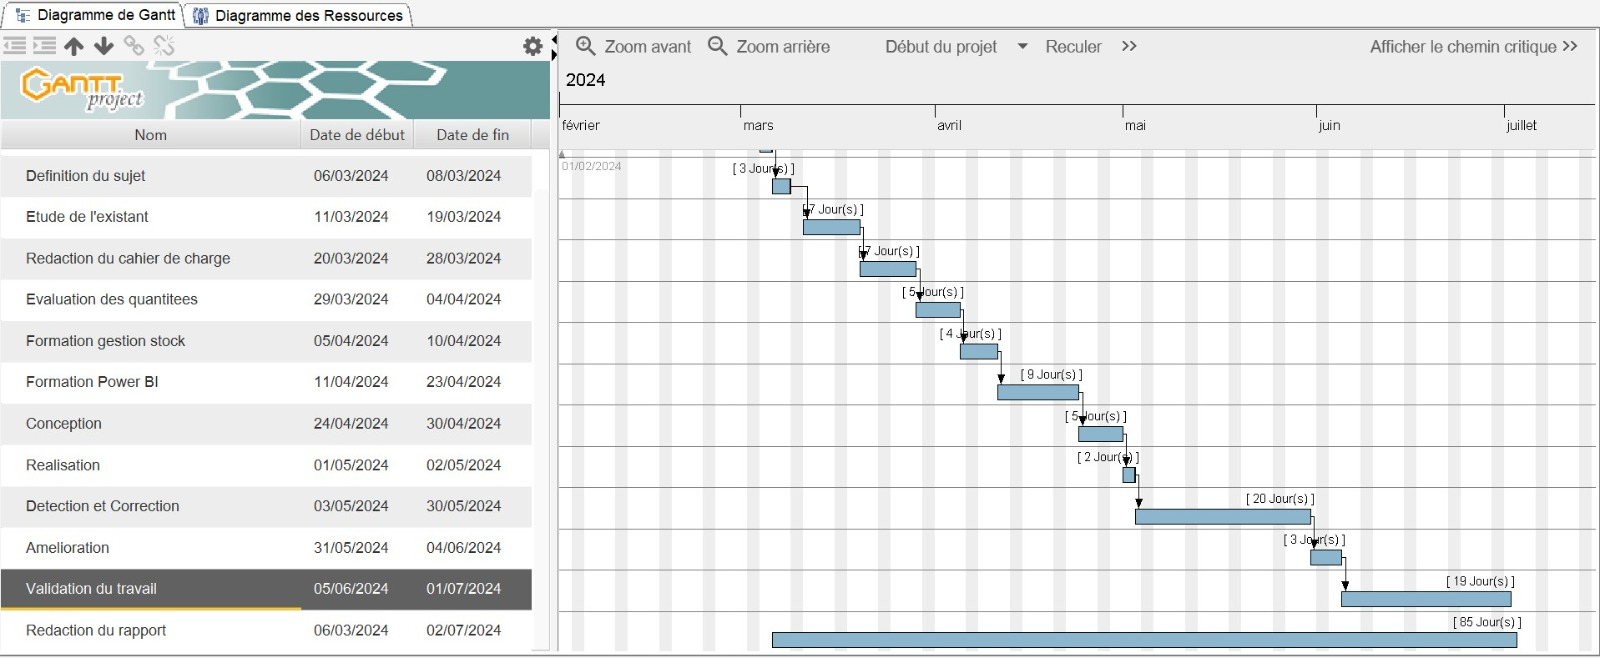
\includegraphics[width=1\textwidth]{images/f1} % Insère l’image avec une largeur égale à 80 % de la largeur du texte
	\caption{Diagramme de Gantt} % Ajoute la légende et le numéro automatique de la figure
	\label{f1} % Donne un identifiant à la figure pour pouvoir la citer dans le texte
\end{figure} % Termine l’environnement de la figure


\begin{figure}[H] % Commence l’environnement de la figure et impose son emplacement ici
	\centering % Centre l’image horizontalement sur la page
	
\includegraphics[width=1\textwidth]{images/ocp} % Insère l’image avec une largeur égale à 80 % de la largeur du texte
	\caption{Image de l'ocp} % Ajoute la légende et le numéro automatique de la figure
	\label{ocp} % Donne un identifiant à la figure pour pouvoir la citer dans le texte
\end{figure} %


\begin{figure}[H] % Commence l’environnement de la figure et impose son emplacement ici
	\centering % Centre l’image horizontalement sur la page
	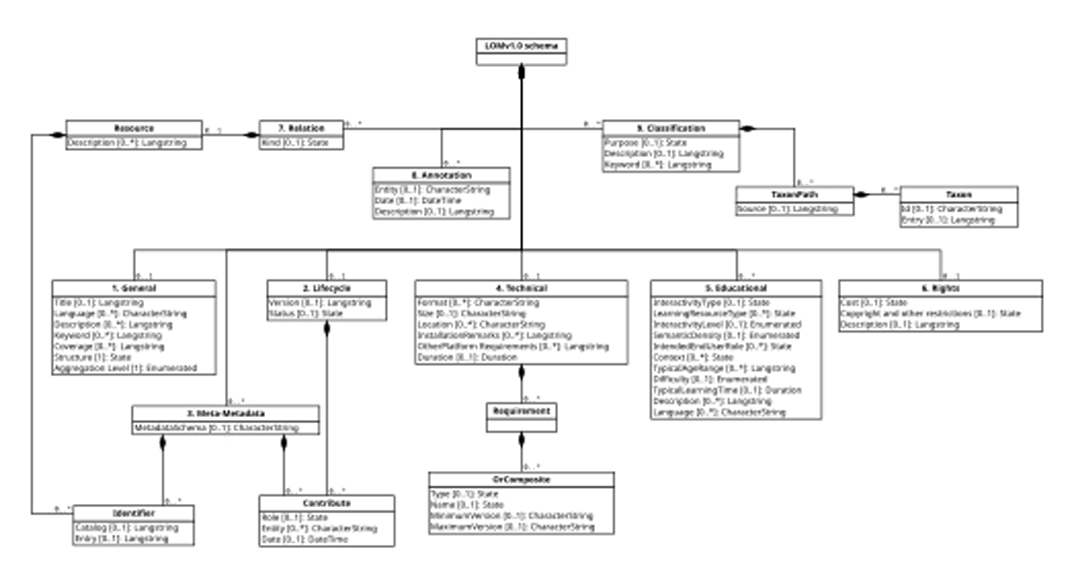
\includegraphics[width=1\textwidth]{images/diag} % Insère l’image avec une largeur égale à 80 % de la largeur du texte
	\caption{Diagramme de classe} % Ajoute la légende et le numéro automatique de la figure
	\label{diag} % Donne un identifiant à la figure pour pouvoir la citer dans le texte
\end{figure} %

La figure \ref{diag} présente le diagramme de classe.\\




La figure \ref{ocp} présente l'image de l'ocp \cite{ocp}.\\
Comme le montre la figure \ref{f1}, un diagramme de Gantt permet de suivre l'avancement des projets, les tâches qui se chevauchent et les dépendances entre elles.

\section{Tableau}
Ce bloc de code insère un tableau sous forme d'image. Le tableau \ref{l1} présente la fiche signalétique du groupe OCP. Ce tableau fournit des informations essentielles sur l'organisation, y compris sa structure et ses principales activités.

\begin{table}[H]
	\centering
	\captionof{table}{Fiche signalétique du groupe OCP}
	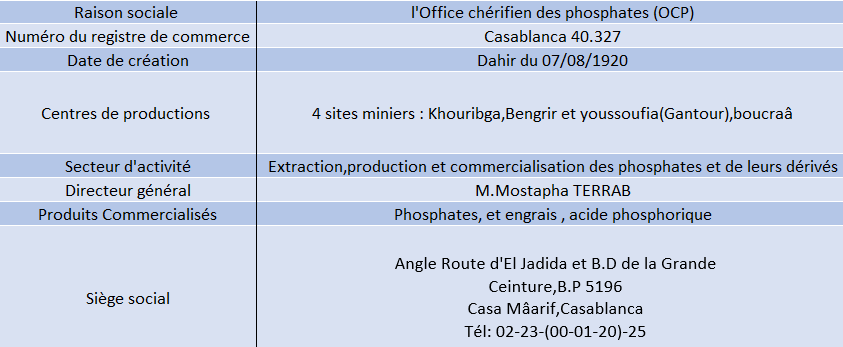
\includegraphics[width=1\textwidth]{images/t1} % Remplacez par le chemin de votre image de tableau
	\label{l1} % Ajout du label pour la référence croisée
\end{table}

\begin{table}[H]
	\centering
	\captionof{table}{Tableau test}
	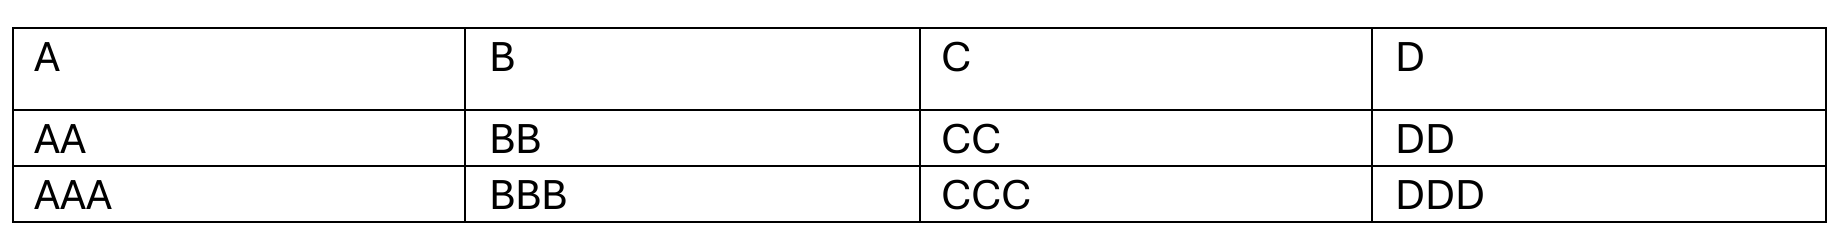
\includegraphics[width=1\textwidth]{images/t2} % Remplacez par le chemin de votre image de tableau
	\label{t2} % Ajout du label pour la référence croisée
\end{table}


\begin{table}[H]
	\centering
	\renewcommand{\arraystretch}{1.2}
	\begin{tabular}{|p{3cm}|p{3cm}|p{3cm}|p{3cm}|}
		\hline
		A   & B   & C   & D   \\ \hline
		AA  & BB  & CC  & DD  \\ \hline
		AAA & BBB & CCC & DDD \\ \hline
	\end{tabular}
\end{table}

Le tableau \ref{t2} présente ... \\
Comme montré dans le tableau \ref{l1}, la fiche signalétique présente les informations clés sur le groupe OCP, telles que sa date de création, son secteur d'activité, et d'autres données importantes.



\section{Conclusion}
xx xxxxx xxxx xxxxx xxxxx xxxxx xxxxxxxxx xxxxx xxxxxxx xxxx xxxxxxxxx xxxxxxx xxxxxx xxxx xxxxxxxxx xxxxxxxx xxxxxxxx xxxxxxxxx xxxxx xxxxxxxxxxx xxxxx xxxxxxx


			\chapter{Cadre théorique de gestion des stocks}
\begin{spacing}{1.2}
\minitoc
\thispagestyle{MyStyle}
\end{spacing}
\newpage

\section{Introduction}
xx xxxxx xxxx xxxxx xxxxx xxxxx xxxxxxxxx xxxxx xxxxxxx xxxx xxxxxxxxx xxxxxxx xxxxxx xxxx xxxxxxxxx xxxxxxxx xxxxxxxx xxxxxxxxx xxxxx xxxxxxxxxxx xxxxx xxxxxxx 
			\chapter{Analyse de l'existant}
\begin{spacing}{1.2}
\minitoc
\thispagestyle{MyStyle}
\end{spacing}
\newpage

\section{Introduction}
xx xxxxx xxxx xxxxx xxxxx xxxxx xxxxxxxxx xxxxx xxxxxxx xxxx xxxxxxxxx xxxxxxx xxxxxx xxxx xxxxxxxxx xxxxxxxx xxxxxxxx xxxxxxxxx xxxxx xxxxxxxxxxx xxxxx xxxxxxx 


\section{Bullet point}

\textbf{•\hspace{0.5cm} XXXX}\\
xx xxxxx xxxx xxxxx xxxxx xxxxx xxxxxxxxx xxxxx xxxxxxx xxxx xxxxxxxxx xxxxxxx xxxxxx xxxx xxxxxxxxx xxxxxxxx xxxxxxxx xxxxxxxxx xxxxx xxxxxxxxxxx xxxxx xxxxxxx 

\section{Conclusion}
xx xxxxx xxxx xxxxx xxxxx xxxxx xxxxxxxxx xxxxx xxxxxxx xxxx xxxxxxxxx xxxxxxx xxxxxx xxxx xxxxxxxxx xxxxxxxx xxxxxxxx xxxxxxxxx xxxxx xxxxxxxxxxx xxxxx xxxxxxx 





			\chapter*{Conclusion générale et perspectives}
\markboth{Conclusion générale}{}
\addcontentsline{toc}{chapter}{Conclusion générale et perspectives}
\adjustmtc
\thispagestyle{MyStyle}
xx xxxxx xxxx xxxxx xxxxx xxxxx xxxxxxxxx xxxxx xxxxxxx xxxx xxxxxxxxx xxxxxxx xxxxxx xxxx xxxxxxxxx xxxxxxxx xxxxxxxx xxxxxxxxx xxxxx xxxxxxxxxxx xxxxx xxxxxxx 

			\addcontentsline{toc}{chapter}{Bibliographie}
\adjustmtc
\renewcommand\bibname{Bibliographie}
\begin{thebibliography}{9}
	\thispagestyle{MyStyle}
	
	\bibitem{ganttproject}
	\textbf{Diagramme de Gantt}.
	\emph{Logiciel libre de gestion et de planification de projets}.
	Disponible à l'adresse :
	\url{https://www.ganttproject.biz/}
	(consulté le 10 Mai 2026).
	
	\bibitem{ocp}
	\textbf{Groupe OCP}.
	\emph{Site officiel du Groupe OCP}.
	Disponible à l'adresse :
	\url{https://www.ocpgroup.ma/fr}
	(consulté le 29 Mai 2026).
	
	\bibitem{managem}
	\textbf{Groupe Managem}.
	\emph{Site officiel du Groupe Managem}.
	Disponible à l'adresse :
	\url{https://www.managemgroup.com/en}
	(consulté le 20 juillet 2026).
	
	\bibitem{vscode}
	\textbf{Visual Studio Code}.
	\emph{Éditeur de code source}.
	Disponible à l'adresse :
	\url{https://code.visualstudio.com/}
	(consulté le 11 juin 2026).
	
	\bibitem{texstudio}
	\textbf{TeXstudio}.
	\emph{Documentation officielle de TeXstudio}.
	Disponible à l'adresse :
	\url{https://www.texstudio.org/}
	(consulté le 06 juillet 2026).
	
\end{thebibliography}


			\chapter*{Annexes}
\markboth{Annexes}{}
\addcontentsline{toc}{chapter}{Annexes}
\adjustmtc
\thispagestyle{MyStyle}

%% add to table of contents : Annexe.1
\makeatletter\renewcommand\thesection{A.\@arabic\c@section}\makeatother

%add spacing in the table of figures
\addtocontents{lof}{\vspace{0.3cm}}

\appendix
\renewcommand{\thefigure}{A.\arabic{figure}}
\setcounter{figure}{0}
\section{Annexe 1 : Schéma électrique de l'installation }
xx xxxxx xxxx xxxxx xxxxx xxxxx xxxxxxxxx xxxxx xxxxxxx xxxx xxxxxxxxx xxxxxxx xxxxxx xxxx xxxxxxxxx xxxxxxxx xxxxxxxx xxxxxxxxx xxxxx xxxxxxxxxxx xxxxx xxxxxxx 


\begin{figure}[H] % Commence l’environnement de la figure et impose son emplacement ici
	\centering % Centre l’image horizontalement sur la page
	
\includegraphics[width=1\textwidth]{images/ocp} % Insère l’image avec une largeur égale à 80 % de la largeur du texte

\end{figure} %
			
		\end{document}